\FloatBarrier
\section[Optimal Curve Reparameterization through Geodesic Interpolation]{Optimal Curve Reparameterization through \\ Geodesic Interpolation}
\label{sec:optimal-curve-reparameterization}

This section presents an optimal reparameterization technique for curve alignment within Lie groups, particularly \(\mathrm{SO}(3)\) and \(\mathrm{SE}(3)\). Unlike the dynamic programming approach in Section \ref{sec:dynamic-programming}, this method provides a continuous framework for curve comparison over the domain \([0,1]\) without a fixed set of nodes. As it does not use the SRVT framework (discussed in \ref{subsec:srvt}), this approach may result in very small geodesic distances for curves of different shapes. It is mainly applied to align curves with assumed identical shapes.

\subsection{Overview of methodology}
\label{subsec:methodology-overview-geodesic-interpolation}

The goal is to reparameterize a discrete curve \(g\) in a Lie group \(G\) to minimize the shape distance to another curve \(h\). This is achieved by identifying a diffeomorphism \(\varphi \in \mathrm{Diff}^+([0,1])\) that transforms \(g\) into \(g_\varphi(t) = g(\varphi(t))\) for \(t \in [0,1]\), aligning it with \(h\) at specific points. Geodesic interpolation facilitates detailed comparisons throughout \([0,1]\), not limited to discrete points.

The alignment's objective function is formulated as:
\begin{equation}
    C(s_k^\varphi) = \sum_{k=0}^N \| \log(g(s_k^\varphi)^{-1} h(s_k)) \|_F^2,
    \label{eq:cost-function-geodesic-interpolation}
\end{equation}
where \(s_k\) are equidistant nodes along \(h\) and \(s_k^\varphi = \varphi(s_k)\) are the transformed nodes of \(g\).

For multi-component curves \(g_i\) and \(h_i\), the function expands to:
\begin{equation}
    C(s_k^\varphi) = \sum_{i=1}^n \sum_{k=0}^N \| \log(g_i(s_k^\varphi)^{-1} h_i(s_k)) \|_F^2,
    \label{eq:cost-function-geodesic-interpolation-cartesian}
\end{equation}
where \(g_i\) and \(h_i\) are the i-th components of the curves \(g\) and \(h\).

Minimizing \(C(s_k^\varphi)\) can be done in several ways, but is here performed using Sequential Least Squares Quadratic Programming (SLSQP) via \texttt{scipy.optimize} \cite{virtanenSciPyFundamentalAlgorithms2020}, ensuring an increasing \(\varphi\) and mitigating local minima with multiple randomized initializations.

\subsection{Numerical Analysis}
\label{subsec:geodesic-interpolation-analysis}

This subsection evaluates the performance of our reparameterization framework on synthetic data. We first reparameterize synthetic curves of the same shape, and then explore its application for classification.

\subsubsection{Reparameterization of Curves}
\label{subsubsec:reparameterization-curves}

For this analysis, we use synthetic data generated as described in \ref{subsec:synthetic-data-generation}. We reparameterize equidistant curves \(c_i^\text{eq}\) and \(c_{i,i+1,i+2}^\text{eq}\) to match parameterized curves \(c_i^j\) and \(c_{i,i+1,i+2}^j\), respectively, as in the dynamic programming approach described in \ref{subsec:reparameterization-curves}. The quality of reparameterization is assessed by comparing the resulting reparameterizations \(\hat{\varphi}_j^i\) with the original parameterizations \(\varphi_j\). 

\begin{figure}[!ht]
    \begin{tikzpicture}
        \begin{axis}[
            width=0.85\textwidth,
            height=0.55\textwidth,
            xlabel={\( x \)},
            ylabel={\( \varphi(x) \)},
            grid=major,
            grid style={dashed,gray!30},
            legend style={at={(1.05,0.5)}, anchor=west},
            line width=1pt,
            xmin=0, xmax=1,
            ymin=0, ymax=1
        ]
        \addplot [thin, red, solid] table [x=x, y=varphi_1, col sep=comma] {figures/syntetic_data/parameterization/varphi_1.csv};
        \addlegendentry{\( \varphi_1\)}

        \addplot [thin, blue, solid] table [x=x, y=varphi_2, col sep=comma] {figures/syntetic_data/parameterization/varphi_2.csv};
        \addlegendentry{\( \varphi_2\)}

        \addplot [thin, green, solid] table [x=x, y=varphi_3, col sep=comma] {figures/syntetic_data/parameterization/varphi_3.csv};
        \addlegendentry{\( \varphi_3\)}


        \addplot [red, dashed] table [x=x, y=g0, col sep=comma] {figures/syntetic_data/reparameterization_SO3_SLERP/df_varphi_1.csv};
        \addlegendentry{\( \hat \varphi_{1}^{1}\)}

        \addplot [red, dotted] table [x=x, y=g1, col sep=comma] {figures/syntetic_data/reparameterization_SO3_SLERP/df_varphi_1.csv};
        \addlegendentry{\( \hat \varphi_{1}^{2}\)}

        \addplot [red, dashdotted] table [x=x, y=g2, col sep=comma] {figures/syntetic_data/reparameterization_SO3_SLERP/df_varphi_1.csv};
        \addlegendentry{\( \hat \varphi_{1}^{3}\)}

        \addplot [blue, dashed] table [x=x, y=g0, col sep=comma] {figures/syntetic_data/reparameterization_SO3_SLERP/df_varphi_2.csv};
        \addlegendentry{\( \hat \varphi_{2}^{1}\)}

        \addplot [blue, dotted] table [x=x, y=g1, col sep=comma] {figures/syntetic_data/reparameterization_SO3_SLERP/df_varphi_2.csv};
        \addlegendentry{\( \hat \varphi_{2}^{2}\)}

        \addplot [blue, dashdotted] table [x=x, y=g2, col sep=comma] {figures/syntetic_data/reparameterization_SO3_SLERP/df_varphi_2.csv};
        \addlegendentry{\( \hat \varphi_{2}^{3}\)}

        \addplot [green, dashed] table [x=x, y=g0, col sep=comma] {figures/syntetic_data/reparameterization_SO3_SLERP/df_varphi_3.csv};
        \addlegendentry{\( \hat \varphi_{3}^{1}\)}

        \addplot [green, dotted] table [x=x, y=g1, col sep=comma] {figures/syntetic_data/reparameterization_SO3_SLERP/df_varphi_3.csv};
        \addlegendentry{\( \hat \varphi_{3}^{2}\)}

        \addplot [green, dashdotted] table [x=x, y=g2, col sep=comma] {figures/syntetic_data/reparameterization_SO3_SLERP/df_varphi_3.csv};
        \addlegendentry{\( \hat \varphi_{3}^{3}\)}

        \end{axis}
    \end{tikzpicture}    
    \caption[Reparameterization of Curves in \(\mathrm{SO}(3)\)]{Comparison of reparameterization results for \(\mathrm{SO}(3)\) data, showing \(\hat{\varphi}_j^{i}\) obtained from our framework versus the analytical \(\varphi_j\). Here, \(j \in \{1, 2, 3\}\) denotes the mappings, and \(i \in \{1, 2, 3\}\) indicates the shapes. Colors represent different mappings, while line styles distinguish the shapes, illustrating the accuracy of the fit.}
    \label{fig:reparameterization-SO3-SLERP}
\end{figure}

\begin{figure}[!ht]
    \begin{tikzpicture}
        \begin{axis}[
            width=0.8\textwidth,
            height=0.55\textwidth,
            xlabel={\( x \)},
            ylabel={\( \varphi(x) \)},
            grid=major,
            grid style={dashed,gray!30},
            legend style={at={(1.05,0.5)}, anchor=west},
            line width=1pt,
            xmin=0, xmax=1,
            ymin=0, ymax=1
        ]
        \addplot [thin, red, solid] table [x=x, y=varphi_1, col sep=comma] {figures/syntetic_data/parameterization/varphi_1.csv};
        \addlegendentry{\( \varphi_1\)}

        \addplot [thin, blue, solid] table [x=x, y=varphi_2, col sep=comma] {figures/syntetic_data/parameterization/varphi_2.csv};
        \addlegendentry{\( \varphi_2\)}

        \addplot [thin, green, solid] table [x=x, y=varphi_3, col sep=comma] {figures/syntetic_data/parameterization/varphi_3.csv};
        \addlegendentry{\( \varphi_3\)}


        \addplot [red, dashed] table [x=x, y=g0, col sep=comma] {figures/syntetic_data/reparameterization_SO3_3_SLERP/df_varphi_1.csv};
        \addlegendentry{\( \hat \varphi_{1}^{(1,2,3)}\)}

        \addplot [red, dotted] table [x=x, y=g1, col sep=comma] {figures/syntetic_data/reparameterization_SO3_3_SLERP/df_varphi_1.csv};
        \addlegendentry{\( \hat \varphi_{1}^{(4,5,6)}\)}

        \addplot [red, dashdotted] table [x=x, y=g2, col sep=comma] {figures/syntetic_data/reparameterization_SO3_3_SLERP/df_varphi_1.csv};
        \addlegendentry{\( \hat \varphi_{1}^{(7,8,9)}\)}

        \addplot [blue, dashed] table [x=x, y=g0, col sep=comma] {figures/syntetic_data/reparameterization_SO3_3_SLERP/df_varphi_2.csv};
        \addlegendentry{\( \hat \varphi_{2}^{(1,2,3)}\)}

        \addplot [blue, dotted] table [x=x, y=g1, col sep=comma] {figures/syntetic_data/reparameterization_SO3_3_SLERP/df_varphi_2.csv};
        \addlegendentry{\( \hat \varphi_{2}^{(4,5,6)}\)}

        \addplot [blue, dashdotted] table [x=x, y=g2, col sep=comma] {figures/syntetic_data/reparameterization_SO3_3_SLERP/df_varphi_2.csv};
        \addlegendentry{\( \hat \varphi_{2}^{(7,8,9)}\)}

        \addplot [green, dashed] table [x=x, y=g0, col sep=comma] {figures/syntetic_data/reparameterization_SO3_3_SLERP/df_varphi_3.csv};
        \addlegendentry{\( \hat \varphi_{3}^{(1,2,3)}\)}

        \addplot [green, dotted] table [x=x, y=g1, col sep=comma] {figures/syntetic_data/reparameterization_SO3_3_SLERP/df_varphi_3.csv};
        \addlegendentry{\( \hat \varphi_{3}^{(4,5,6)}\)}

        \addplot [green, dashdotted] table [x=x, y=g2, col sep=comma] {figures/syntetic_data/reparameterization_SO3_3_SLERP/df_varphi_3.csv};
        \addlegendentry{\( \hat \varphi_{3}^{(7,8,9)}\)}
        \end{axis}
    \end{tikzpicture}    
    \caption[Reparameterization of Curves in \(\mathrm{SO}(3)^3\)]{Comparison of reparameterization results for \(\mathrm{SO}(3)^3\) data, showing \(\hat{\varphi}_j^{i,i+1,i+2}\) obtained from our framework versus the analytical \(\varphi_j\). Here, \(j \in \{1, 2, 3\}\) denotes the mappings, and \(i \in \{1, 4, 7\}\) indicates the shapes. Colors represent different mappings, while line styles distinguish the shapes, illustrating the accuracy of the fit.}
    \label{fig:reparameterization-SO3-3-SLERP}
\end{figure}

\begin{figure}[!ht]
    \begin{tikzpicture}
        \begin{axis}[
            width=0.85\textwidth,
            height=0.55\textwidth,
            xlabel={\( x \)},
            ylabel={\( \varphi(x) \)},
            grid=major,
            grid style={dashed,gray!30},
            legend style={at={(1.05,0.5)}, anchor=west},
            line width=1pt,
            xmin=0, xmax=1,
            ymin=0, ymax=1
        ]
        \addplot [thin, red, solid] table [x=x, y=varphi_1, col sep=comma] {figures/syntetic_data/parameterization/varphi_1.csv};
        \addlegendentry{\( \varphi_1\)}

        \addplot [thin, blue, solid] table [x=x, y=varphi_2, col sep=comma] {figures/syntetic_data/parameterization/varphi_2.csv};
        \addlegendentry{\( \varphi_2\)}

        \addplot [thin, green, solid] table [x=x, y=varphi_3, col sep=comma] {figures/syntetic_data/parameterization/varphi_3.csv};
        \addlegendentry{\( \varphi_3\)}

        \addplot [red, dashed] table [x=x, y=g0, col sep=comma] {figures/syntetic_data/reparameterization_SE3_SLERP/df_varphi_1.csv};
        \addlegendentry{\( \hat \varphi_{1}^1\)}

        \addplot [red, dotted] table [x=x, y=g1, col sep=comma] {figures/syntetic_data/reparameterization_SE3_SLERP/df_varphi_1.csv};
        \addlegendentry{\( \hat \varphi_{1}^2\)}

        \addplot [red, dashdotted] table [x=x, y=g2, col sep=comma] {figures/syntetic_data/reparameterization_SE3_SLERP/df_varphi_1.csv};
        \addlegendentry{\( \hat \varphi_{1}^3\)}

        \addplot [blue, dashed] table [x=x, y=g0, col sep=comma] {figures/syntetic_data/reparameterization_SE3_SLERP/df_varphi_2.csv};
        \addlegendentry{\( \hat \varphi_{2}^1\)}

        \addplot [blue, dotted] table [x=x, y=g1, col sep=comma] {figures/syntetic_data/reparameterization_SE3_SLERP/df_varphi_2.csv};
        \addlegendentry{\( \hat \varphi_{2}^2\)}

        \addplot [blue, dashdotted] table [x=x, y=g2, col sep=comma] {figures/syntetic_data/reparameterization_SE3_SLERP/df_varphi_2.csv};
        \addlegendentry{\( \hat \varphi_{2}^3\)}

        \addplot [green, dashed] table [x=x, y=g0, col sep=comma] {figures/syntetic_data/reparameterization_SE3_SLERP/df_varphi_3.csv};
        \addlegendentry{\( \hat \varphi_{3}^1\)}

        \addplot [green, dotted] table [x=x, y=g1, col sep=comma] {figures/syntetic_data/reparameterization_SE3_SLERP/df_varphi_3.csv};
        \addlegendentry{\( \hat \varphi_{3}^2\)}

        \addplot [green, dashdotted] table [x=x, y=g2, col sep=comma] {figures/syntetic_data/reparameterization_SE3_SLERP/df_varphi_3.csv};
        \addlegendentry{\( \hat \varphi_{3}^3\)}

        \end{axis}
    \end{tikzpicture}    
    \caption[Reparameterization of Curves in \(\mathrm{SE}(3)\)]{Comparison of reparameterization results for \(\mathrm{SE}(3)\) data, showing \(\hat{\varphi}_j^{i}\) obtained from our framework versus the analytical \(\varphi_j\). Here, \(j \in \{1, 2, 3\}\) denotes the mappings, and \(i \in \{1, 2, 3\}\) indicates the shapes. Colors represent different mappings, while line styles distinguish the shapes, illustrating the accuracy of the fit.}
    \label{fig:reparameterization-SE3-SLERP}
\end{figure}

\begin{figure}[!ht]
    \begin{tikzpicture}
        \begin{axis}[
            width=0.8\textwidth,
            height=0.55\textwidth,
            xlabel={\( x \)},
            ylabel={\( \varphi(x) \)},
            grid=major,
            grid style={dashed,gray!30},
            legend style={at={(1.05,0.5)}, anchor=west},
            line width=1pt,
            xmin=0, xmax=1,
            ymin=0, ymax=1
        ]
        \addplot [thin, red, solid] table [x=x, y=varphi_1, col sep=comma] {figures/syntetic_data/parameterization/varphi_1.csv};
        \addlegendentry{\( \varphi_1\)}

        \addplot [thin, blue, solid] table [x=x, y=varphi_2, col sep=comma] {figures/syntetic_data/parameterization/varphi_2.csv};
        \addlegendentry{\( \varphi_2\)}

        \addplot [thin, green, solid] table [x=x, y=varphi_3, col sep=comma] {figures/syntetic_data/parameterization/varphi_3.csv};
        \addlegendentry{\( \varphi_3\)}


        \addplot [red, dashed] table [x=x, y=g0, col sep=comma] {figures/syntetic_data/reparameterization_SE3_3_SLERP/df_varphi_1.csv};
        \addlegendentry{\( \hat \varphi_{1}^{(1,2,3)}\)}

        \addplot [red, dotted] table [x=x, y=g1, col sep=comma] {figures/syntetic_data/reparameterization_SE3_3_SLERP/df_varphi_1.csv};
        \addlegendentry{\( \hat \varphi_{1}^{(4,5,6)}\)}

        \addplot [red, dashdotted] table [x=x, y=g2, col sep=comma] {figures/syntetic_data/reparameterization_SE3_3_SLERP/df_varphi_1.csv};
        \addlegendentry{\( \hat \varphi_{1}^{(7,8,9)}\)}

        \addplot [blue, dashed] table [x=x, y=g0, col sep=comma] {figures/syntetic_data/reparameterization_SE3_3_SLERP/df_varphi_2.csv};
        \addlegendentry{\( \hat \varphi_{2}^{(1,2,3)}\)}

        \addplot [blue, dotted] table [x=x, y=g1, col sep=comma] {figures/syntetic_data/reparameterization_SE3_3_SLERP/df_varphi_2.csv};
        \addlegendentry{\( \hat \varphi_{2}^{(4,5,6)}\)}

        \addplot [blue, dashdotted] table [x=x, y=g2, col sep=comma] {figures/syntetic_data/reparameterization_SE3_3_SLERP/df_varphi_2.csv};
        \addlegendentry{\( \hat \varphi_{2}^{(7,8,9)}\)}

        \addplot [green, dashed] table [x=x, y=g0, col sep=comma] {figures/syntetic_data/reparameterization_SE3_3_SLERP/df_varphi_3.csv};
        \addlegendentry{\( \hat \varphi_{3}^{(1,2,3)}\)}

        \addplot [green, dotted] table [x=x, y=g1, col sep=comma] {figures/syntetic_data/reparameterization_SE3_3_SLERP/df_varphi_3.csv};
        \addlegendentry{\( \hat \varphi_{3}^{(4,5,6)}\)}

        \addplot [green, dashdotted] table [x=x, y=g2, col sep=comma] {figures/syntetic_data/reparameterization_SE3_3_SLERP/df_varphi_3.csv};
        \addlegendentry{\( \hat \varphi_{3}^{(7,8,9)}\)}

        \end{axis}
    \end{tikzpicture}    
    \caption[Reparameterization of Curves in \(\mathrm{SE}(3)^3\)]{Comparison of reparameterization results for \(\mathrm{SE}(3)^3\) data, showing \(\hat{\varphi}_j^{i,i+1,i+2}\) obtained from our framework versus the analytical \(\varphi_j\). Here, \(j \in \{1, 2, 3\}\) denotes the mappings, and \(i \in \{1, 4, 7\}\) indicates the shapes. Colors represent different mappings, while line styles distinguish the shapes, illustrating the accuracy of the fit.}
    \label{fig:reparameterization-SE3-3-SLERP}
\end{figure}

The effectiveness of these reparameterizations is visually demonstrated in Figures \ref{fig:reparameterization-SO3-SLERP}, \ref{fig:reparameterization-SO3-3-SLERP}, \ref{fig:reparameterization-SE3-SLERP}, and \ref{fig:reparameterization-SE3-3-SLERP}. These figures show alignment improvements, where true parameterizations are represented by solid lines, and reparameterization results by dashed, dotted, and dash-dotted lines. Colors indicate shapes, and line styles represent mappings.

The results show that the reparameterization framework aligns the curves well with the true parameterizations. The curves are closely matched, demonstrating the method's effectiveness. While some discrepancies are observed, especially in Figure \ref{fig:reparameterization-SO3-SLERP}, this may be due to local minima or insufficient runtime due to the method's computational expense, and should be further investigated.

\subsubsection{Classification of Curves}
\label{subsubsec:classification-curves}

We use the same synthetic data to classify curves based on their shapes. The classification is performed by computing the shape space distance between the curves using the cost functions \eqref{eq:cost-function-geodesic-interpolation} and \eqref{eq:cost-function-geodesic-interpolation-cartesian}. We store the cost between each pair of curves in a distance matrix. The distance matrix is visualized through heatmaps, where color intensity indicates the shape space distance between the curves, as shown in Figures \ref{fig:classification-SO3-interpolation} and \ref{fig:classification-SE3-interpolation}. We did not perform this classification on the curves in \(\mathrm{SE}(3)^3\) and \(\mathrm{SO}(3)^3\) due to the high computational expense and the method's unsuitability for comparing curves of different shapes.

\begin{figure}[!ht]
    \centering
    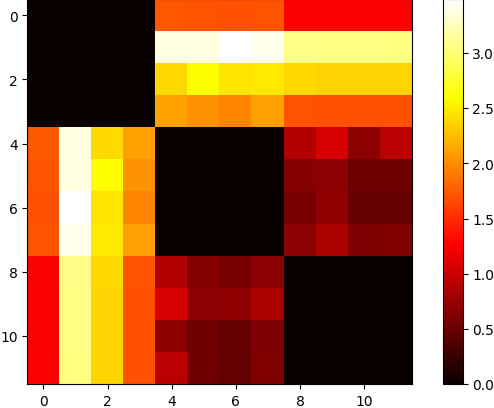
\includegraphics[width=0.6\linewidth]{figures/syntetic_data/distance_matrix/SO3_interpolation}
    \caption[Classification using interpolation to reparameterization of curves in \(\mathrm{SO}(3)\)]{Classification of synthetic \(\mathrm{SO}(3)\) curves across 100 timesteps, with geodesic interpolation to reparameterize, depicted as a distance matrix of twelve curves, denoted \(c_i^j\), where \(i = 1, 2, 3\) and \(j = 1, 2, 3, 4\). The color intensity within the matrix indicates the shape space distance.}
    \label{fig:classification-SO3-interpolation}
\end{figure}

\begin{figure}[!ht]
    \centering
    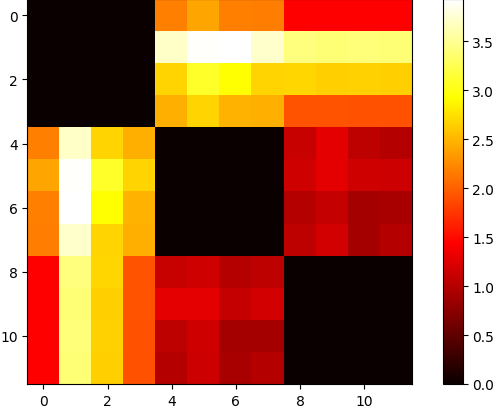
\includegraphics[width=0.6\linewidth]{figures/syntetic_data/distance_matrix/SE3_interpolation}
    \caption[Classification using interpolation to reparameterization of curves in \(\mathrm{SE}(3)\)]{Classification of synthetic \(\mathrm{SE}(3)\) curves across 100 timesteps, with geodesic interpolation to reparameterize, illustrated as a distance matrix of twelve curves, denoted \(c_i^j\), where \(i = 1, 2, 3\) and \(j = 1, 2, 3, 4\). The color intensity within the matrix indicates the shape space distance.}
    \label{fig:classification-SE3-interpolation}
\end{figure}

\FloatBarrier
As seen in the heatmaps, the classification is successful, with almost zero intra-class distances and high inter-class distances. This indicates that the curves are well separated in the shape space, and the classification is accurate. While these results are promising, we refrain from using this method for classifying motion capture data due to uncertainties about its robustness.